% !TEX root = ../main.tex
\subsection*{Life in the Poleis} \label{ssec::lifeinthepoleis}
Civilization in Viphoger is centered in three poleis: Akhosh, Mephetis, and Setesh.
These poleis exemplify the kins' drive to settle the land, to shape nature according to their needs, and to organize into political structures that can withstand the changing fortunes of the passing centuries.

Each polis is centered in a city but includes a wide region of surrounding territory, and each one has its own distinct society and culture.
To the people of Viphoger, ``Mephetis'' is more or less synonymous with ``Mephetians'' --- the polis isn't just the people who live in the city of Mephetis or even those who dwell in nearby villages; it is the people who follow the Mephetian way of life, wherever they might be found.

% \thispagestyle{empty} % Remove footer so that it doesn't clash with the image.
% \begin{tikzpicture}[remember picture,overlay]
%     \node[anchor=south west, xshift=-0.10cm, yshift=-0.10cm] at (current page.south west) {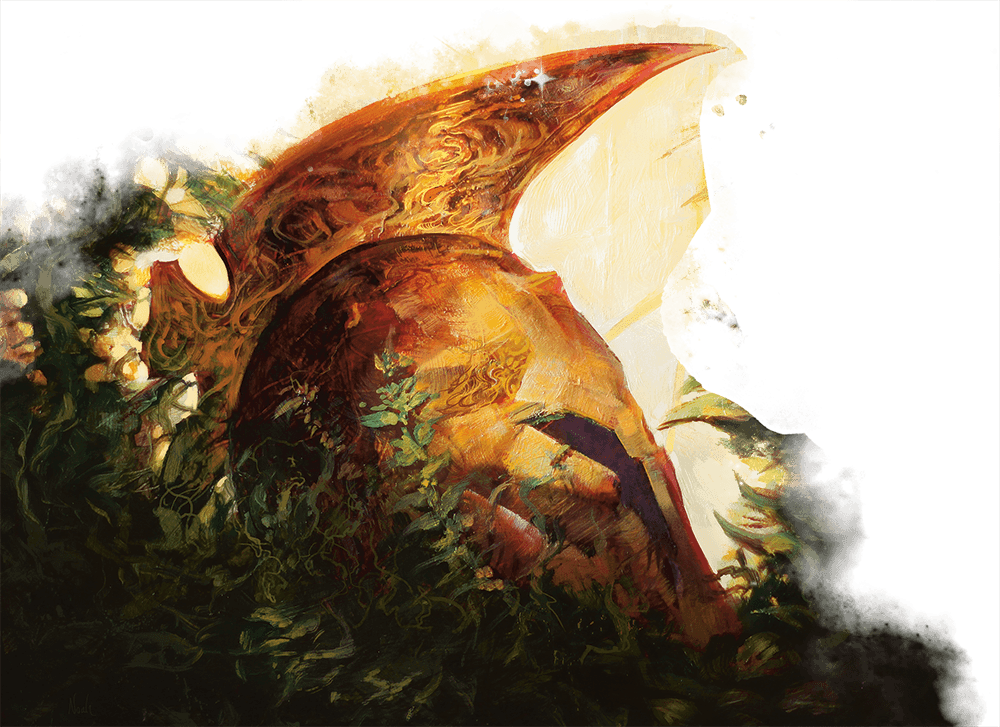
\includegraphics[width=0.5\pdfpagewidth]{02viphoger/img/00hoplite_helmet.png}};
% \end{tikzpicture}

\subsubsection{Citizenship and Government}
In every polis, civic responsibility and full protection are afforded only to citizens.
Citizenship is limited to those whose parents were both citizens of the polis.
Citizens of other poleis, and their children, aren't permitted to participate in the government of the polis.
In Akhosh, citizens must meet one additional requirement: they must serve in the army.

The three poleis have different political structures, but each one has a council elected by popular vote of the citizenry.
The Twelve, Mephetis's council of philosophers, is the democratically elected ruling body of the polis.
Akhosh is ruled by a hereditary monarch who is advised by a council of elders elected by and from among the citizenry.
Similarly, Setesh's Ruling Council is formed by popular vote, and they govern the polis while its queen --- the goddess Karametra --- is absent.

\subsubsection{Trade and Currency}
Trade between Akhosh and Mephetis is constant and productive.
Caravans make the two-week journey between the poleis twice a month, aided by the Tsher river.

They carry fine Akhoash metalwork and pottery to Mephetis, and Mephetian fabric, stonework, and fish westward.
Both poleis mint coins of copper and nickel, with equivalent value.

Setesh trades with the other poleis as well, but less extensively.
Its Abora Market, just inside the city gates, is open to outsiders only on certain days, and Seteshan merchants prefer to barter goods rather than accept currency.
Despite these restrictions, Seteshan food, woodwork, and trained falcons are highly valued in the other poleis.

Aside from the other poleis, Mephetis and Setesh both trade with the dratl irds of the Vahagha band.
The irds don't work metal, so they trade woodwork, the produce of the plains, and woven blankets to the human poleis in exchange for weapons and armor.

\subsubsection{Recreation}
% The people of the poleis enjoy the opportunity for some recreation, as time and money allow.

Gymnasia are popular gathering places, offering athletic training as well as space for philosophical discussion and friendly socializing.
A resident of the city might visit a gymnasium one day to exercise, the next to view a wrestling match between celebrated competitors, and the next to hear a renowned philosopher give a lecture on ethics.

Another important venue for recreation is the theater.
The works of celebrated playwrights, past and present, are regularly produced by casts of professional actors.
On occasion, a storyteller, accompanied by a small orchestra, draws crowds to a theater for a recitation of one of the great epics, such as The Sylvan Wars, The Theriad, or The Callapheia.
Such a performance might stretch over two or three days.

\subsubsection{Independence \& Isolationism}
Mephetis was founded in 476 AS as an imponent bastion against the empire of Hulnar during the Sylvan Wars.
% The polis was erected by the heroes Kynaios and Tiro, marking the end of the et Agnomakhos's reign over the region.
% Despite the fervient attacks of the dratl irds, Mephetis stood its ground against all odds and served as the main fortress of Khedrat during the Sylvan Wars.
As the war ended however, Mephetis --- and the other poleis --- begrudgingly remained under the rule of Khedrat.
Under heavy taxation and limiting regulations, the poleis silently planned their rebellion.

% Tensions quickly rose however when Khedrat's king, Olag the Immortal, banned the colonies for celebrating their religion, Therism.
During the last week of the last month of 659 AS, Mephetian forces snuck into Avshen's port, sparking the One-Week War.
With great cunning and force they crippled the Khedratian military, and were gone as quickly as they arrived.

Impaired, Olag was forced to accept the colonies's independence.
However, this victory didn't come without a price.
So far no nation has established commerce with Viphoger.
Not only due to the country's infamous attack, but also in fear of the shamed Khedrat's retaliation.

\newpage
